\ssection{O Centro de Tecnologia}
    \ssubsection{Mapa e os diferentes blocos}
        Há diferentes cursos de Engenharia distribuídos nos blocos do CT, como você deve saber. Nosso curso, em particular, fica no bloco H, junto com Engenharia Elétrica, Engenharia Nuclear, Engenharia de Controle e Automação e Engenharia de Computação e Informação, sendo as duas últimas mais conhecidas como ECA e ECI, respectivamente. Abaixo, está uma relação dos blocos e suas Engenharias.   
        \begin{table} [!h]
        \centering
        \begin{tabular}{c | l} 
        Bloco & Cursos \\
        \hline
        A & Institutos de Física e Química \\
        B & Biblioteca do CT e Instituto de Matemática\\
        C & Instituto de Matemática e Engenharia Naval\\
        D & Engenharias Ambiental e Civil \\ 
        E & Escola de Química \\
        F & Engenharias de Produção, Metalúrgica e de Materiais \\
        G & Engenharia Mecânica \\
        H & Engenharias Eletrônica e de Computação, Elétrica, \\
        & Controle e Automação (ECA), Computação e Informação (ECI) e Nuclear \\       
        I & COPPE e Laboratórios diversos
        \end{tabular}
        \end{table}

        Para facilitar, você pode ver a localização dos blocos no mapa abaixo:
        
        \begin{center}        	
            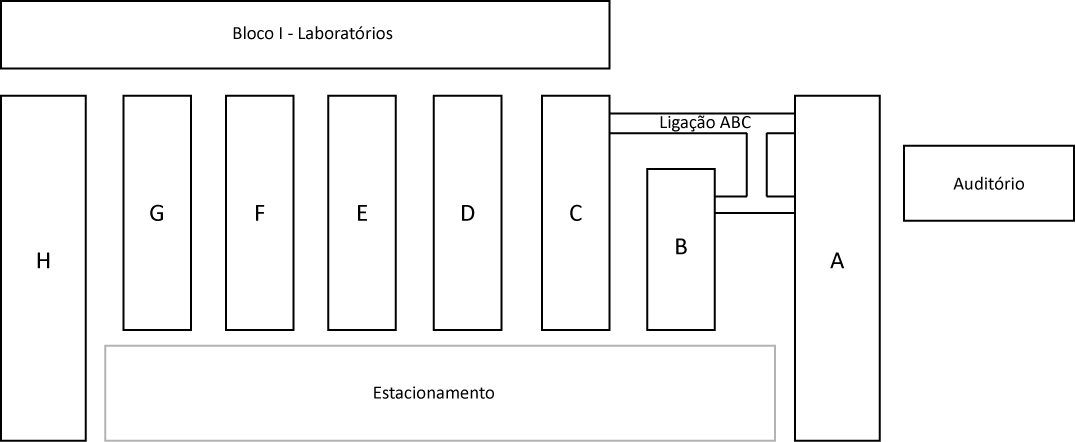
\includegraphics[width=\textwidth]{assets/mapa-ct.png}
            \captionof{figure}{Mapa do Centro de Tecnologia}
        \end{center}

    \ssubsection{Salas de Estudo}
      Com o tempo, você irá perceber a importância desses lugares durante a sua graduação. Apesar do tamanho do CT, não existem muitas salas de estudo por lá e, as poucas que têm, podem ficar muito cheias. 

      Nosso bloco tem uma excelente sala de estudos no $3^o$ andar. Há um ambiente dentro dessa sala conhecido como "sala do silêncio"; em geral, essa regra é muito bem respeitada lá e, por conta disso, se você estiver estudando em grupo, opte por ficar na parte exterior da sala. 

      Abaixo, segue uma lista de ambientes ideais para estudar:
      \begin{itemize}
        \item Sala de estudos no $3^o$ andar do Bloco H -- ar condicionado, tomadas e grande capacidade para alunos
        \item Sala do GECOM -- ar condicionado, tomadas, quadro branco com pilot(!) e ambiente mais descontraído
        \item Biblioteca do bloco B  
      \end{itemize}
      Algumas dicas extras: 
      \begin{itemize}
        \item Salas de estudo ficam muito cheias em dias de provas unificadas (provas comuns à todas as engenharias).
        \item Geralmente, abrem 7h00 e fecham 19h00, mas não é regra geral.
        \item Ajude a conservar nossas salas de estudo não escrevendo nas mesas e jogando seu lixo na lixeira. Não precisava nem falar, mas não custa nada reforçar, né.
      \end{itemize}
    \ssubsection{Biblioteca do CT}
      Para poder pegar livros emprestados, é preciso ir à biblioteca e fazer um cadastro em um dos computadores que ficam disponíveis para isso. Há algumas regras quanto à devolução dos livros e à entrada na biblioteca com itens pessoais, então fique atento!
      \subsection{Dicas}
      \begin{itemize}
      	\item Evite pegar os elevadores do bloco A. Nunca se sabe quando eles podem parar (ocorre com frequência). Use as escadas atrás deles.
      \end{itemize}